\documentclass[fontsize=11pt,paper=a4]{scrartcl}

\usepackage[english]{babel}
\usepackage{microtype}
\usepackage{listings}
\usepackage{hyperref}
\usepackage{csquotes}
\usepackage{graphicx}

\lstset{
  language=C,
  basicstyle=\small,
  breaklines=true
}
\frenchspacing 

%%% Maketitle metadata
\newcommand{\horrule}[1]{\rule{\linewidth}{#1}} 	

\title{
		%\vspace{-1in} 	
		\usefont{OT1}{bch}{b}{n}
		\normalfont \normalsize \textsc
		{Coursera Course: Cloud Computing} \\ [25pt]
		\horrule{0.5pt} \\[0.4cm]
		\huge Capstone Project Task 2 Report \\
		\horrule{2pt} \\[0.5cm]
}
\author{
		\normalfont 	\normalsize
        Hang Shi\\[-3pt] \normalsize        
}
\date{\today}

\begin{document}
\maketitle
		
\section{Overview}
This report covers the design and implementation details for Cloud Computing Captone Project Task 2. The goals of this task are to perform the following:
\begin{itemize}
\item Extract and clean the transportation dataset, and then store the result in HDFS.
\item Answer 2 questions from Group 1, 3 questions from Group 2, and Question 3.2 using Spark. Store the results for questions from Group 2 and Question 3.2 in Cassandra.   
\end{itemize} 
\section{Data Cleanup}
The first task is to clean and store the dataset. We  first retrieve and extract the dataset from the EBS volume snapshot by following steps in \url{http://docs.aws.amazon.com/AWSEC2/latest/UserGuide/ebs-restoring-volume.html}. One key thing to note is that we need to create EC2 instance in the same region and availabbility zone as the data EBS snapshot (snap-e1608d88 in us-east-1d).   

Afterwards, we explore the data set and decide on how we wish to clean it. Then we ignore unrelated rows and extract only the columns from the csv files. The raw data is in \path{/data/aviation/airline_ontime} directory. 

Python and Bash scripts are developed used to do the cleanup: 
\begin{itemize} 
\item A python script is developed on top of \href{https://docs.python.org/2/library/csv.html}{python CSV package} to extract the fields. 
\item Bash scripts are used to loop through all data sets. 
\end{itemize}

Such data cleanup is a one-time job. The cleaned data are stored on HDFS via below hdfs dfs command  as tab delimetered fields with each line indicating one flight. For question 3.2, only 2008 data is used. 
\begin{lstlisting}{centered}
	Cmd: hdfs dfs -copyFromLocal <local files> <hdfs dir>  
	Fields: Year, Month, Day, Weekday, FullDate, Airline, Carrier, Flight, Origin, Dest, CRSDepTime, DepDelay, ArrDelay
\end{lstlisting}

\section{System Overview}
See figure 1 for system architecture details for this project. 
\begin{figure}
\centering
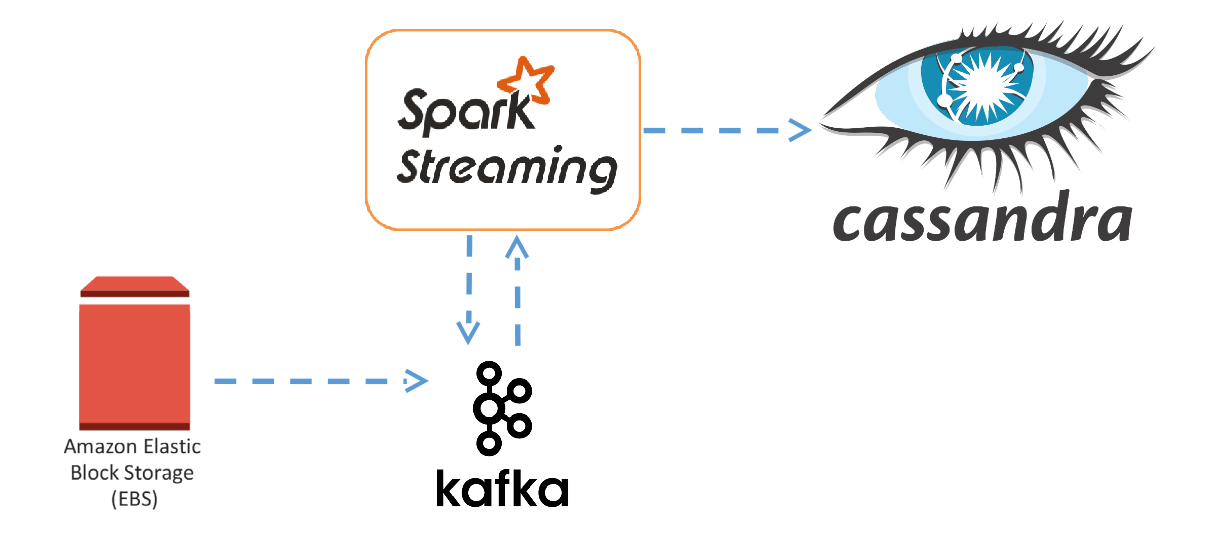
\includegraphics[width=\linewidth,,keepaspectratio]{system_architecture.png}
\caption{System Architecture for This Project.}
\label{fig:verticalcell}
\end{figure}
\subsection{Hadoop, Kafka, and Spark Streaming}
The system is essentially a 4 node Apache Hadoop cluster with one namenode and three datanodes running on AWS EC2. Hadoop Yarn runs and serves as the resource manager and application manager. Kafka is used to stream the cleaned data stored in HDFS to Spark, which does the RDD/Data Frame processing before storing the results to NoSQL database. See below link for details on how to set up and run Spark on EC2. 
\href{https://spark.apache.org/docs/1.6.2/ec2-scripts.html}{Running Spark on EC2}
\subsection{NOSQL Database: Cassandra} 
Cassandra cluster is deployed on the three Hadoop datanodes to provide data replication and scalability. The cluster run on the same rack and utilizes GossipingPropertyFileSnitch scheme. One of the nodes is assigned as the seed provider. Initially version 3.6 is used, but due to the support of group by is missing in 3.6, version 3.11 is used. 

Cassandra Async Batch operation and Data Frame API have been used to insert/update data with Batch operation having less memory requirements, and query scripts are written via Python Cassandra API as well, \href{http://docs.datastax.com/en/drivers/python/3.2/index.html}{Cassandra Python Driver}. 


\section{Group 1 Problems} 
\begin{itemize} 
\item Problem 1.1: Rank the top 10 most popular airports by numbers of flights to/from the airport.
\item Problem 1.2: Rank the top 10 airlines by on-time arrival performance
\end{itemize}
\textbf{Solution:} both problems are solved using same technique: stateful updates via Spark API updateStateByKey. See below for details. 
\begin{lstlisting}[basicstyle=\small,language = python] 
def updateFunction(newValues, runningCount):
    return sum(newValues, runningCount or 0)
filtered = lines.map(lambda line: line.split("\t"))\
                .flatMap(lambda w: [(w[3], 1), (w[4], 1)] )\
                .reduceByKey(lambda a, b: a+b)\
                .updateStateByKey(updateFunction)\
                .transform(lambda r: r.sortBy(lambda (w, c): -c))
\end{lstlisting}
\section{Group 2 Problems}
\begin{itemize} 
\item Problem 2.1: For each airport X, rank the top-10 carriers in decreasing order of on-time departure performance from X. 
\item Problem 2.2: For each airport X, rank the top-10 airports in decreasing order of on-time departure performance from X.
\item Problem 2.3: For each source-destination pair X-Y, rank the top-10 carriers in decreasing order of on-time arrival performance at Y from X.
\item Problem 2.4: For each source-destination pair X-Y, determine the mean arrival delay (in minutes) for a flight from X to Y.
\end{itemize}
\textbf{Solution:} All four questions are solved using same approach: Spark stateful RDD transformation, Data Frame API, and Cassandra Spark API. See below two code examples from problem 2.2. Other questions are similar. 
\begin{lstlisting}[basicstyle=\small,language = python] 
# RDD Processing
def updateFunction(newValues, runningCount):
    values, counter, avg_delay = runningCount or (0., 0, 0.)
    for val in newValues: 
        values += val[0]
        counter += val[1]
    return (values, counter, values/counter) 
f1 = lines.map(lambda line:line.split(","))\
          .map(lambda f:Flight(f))\
          .map(lambda f:((f.Origin, f.Dest),(f.DepDelay, 1)))\
          .updateStateByKey(updateFunction)
filtered = f1.map(lambda (x, y):(x[0], y[2], x[1]))
filtered.foreachRDD(lambda rdd:print_rdd(rdd))
\end{lstlisting}

\begin{lstlisting}[basicstyle=\small,language = python] 
# Data Frame Transformation and Data Storing 
schema = StructType([
         StructField("origin", StringType(), True),
         StructField("delay", FloatType(), True), 
         StructField("dest", StringType(), True)
         ])
df = getSqlContextInstance(rdd.context).createDataFrame(rdd, schema);  
df.show() 
#insert into cassandra 
df.write.format("org.apache.spark.sql.cassandra")\
    .mode('overwrite').options(table="g2e2", keyspace="test")\
    .save()
\end{lstlisting}
\textbf{Data Model or Cassandra Table Definitions: }
\begin{lstlisting}[basicstyle=\small,language = sql] 
CREATE TABLE test.g2e1 (origin text, delay float, airline text, carrier text, PRIMARY KEY (origin, airline) ); 
CREATE TABLE test.g2e2 (origin text, delay float, dest text, PRIMARY KEY (origin, dest) ); 
CREATE TABLE test.g2e3 (origin text, dest text, delay float, airline text, PRIMARY KEY ((origin, dest), airline)); 
CREATE TABLE test.g2e4 (origin text, dest text, delay float, PRIMARY KEY (origin, dest)); 
\end{lstlisting}
\section{Group 3, Problem 3.2}
\begin{itemize}
\item Problem 3.2. Tom wants to travel from airport X to airport Z. However, Tom also wants to stop at airport Y for some sightseeing on the way. More concretely, Tom has the following requirements (see Task 1 Queries for specific queries):
\begin{itemize}
\item A. The second leg of the journey (flight Y-Z) must depart two days after the first leg (flight X-Y). For example, if X-Y departs January 5, 2008, Y-Z must depart January 7, 2008.
\item B. Tom wants his flights scheduled to depart airport X before 12:00 PM local time and to depart airport Y after 12:00 PM local time.
\item C. Tom wants to arrive at each destination with as little delay as possible.
\end{itemize}
\end{itemize}
\textbf{Solution:} First the dataset is mapped into two dataset f{\_}xy and f{\_}yz based on whether the departure time is earlier than 12:00. During f{\_}yz processing, the departure date is substracted two days. Then the two dataset are joined together with origin of f{\_}xy and destination of f{\_}yz are the same, and dates are two days apart. The results are stored into Cassandra database using same approach as in group 2 problems. The primary and cluster keys are days combined with airport and delay, like "PHX{\_}JFK{\_}MSP{\_}2008-09-07". 
\begin{lstlisting}[basicstyle=\small,language = python] 
def map_xy(f): 
    fdate = datetime.date(f.Year, f.Month, f.Day)
    return ((str(fdate), f.Dest), f)
def map_yz(f):
    fdate = datetime.date(f.Year, f.Month, f.Day)
    fdate -= datetime.timedelta(days=2)
    return ((str(fdate), f.Origin), f)
def process_record(record): 
    f_xy = record[1][0]
    f_yz = record[1][1]
    route = '_'.join((f_xy.Origin, f_xy.Dest, f_yz.Dest, record[0][0]))
    delay =  f_xy.ArrDelay + f_yz.ArrDelay
    details = "%s;%s" % (f_xy, f_yz)
    return (route, delay, f_xy.FlightNum, f_yz.FlightNum, details)    
# RDD Processing
f_xy = ff.map(map_xy).filter(lambda (k,v): v.CRSDepTime < '1200')
f_yz = ff.map(map_yz).filter(lambda (k,v): v.CRSDepTime > '1200')

f_xyz = f_xy.join(f_yz).map(process_record) 
f_xyz.foreachRDD(lambda rdd: print_rdd(rdd))
\end{lstlisting}
\textbf{Data Model or Cassandra Table Definitions: }
\begin{lstlisting}[basicstyle=\small,language = sql] 
CREATE TABLE test.g3e2 (route text, delay float, details text, f1 text, f2 text, PRIMARY KEY (route, f1, f2));  
\end{lstlisting} 
\section{Optimization and Discussion}
\begin{itemize}
\item Removal of unused data columns: only needed columns have been imported from the original dataset, thus lowering the needs for data transfer and storage capacity.
\item Data ordering and partitioning: the import script orders and partitions by date the data from the original dataset. This way the import process into HDFS is faster.
\item Data preload into HDFS: data  is loaded to HDFS before starting to process it. This way, we can achieve persistent storage in HDFS and fast access from HDFS.
\item During Kafka streaming, the Spark executor can't handle full speed of Kafka streaming, two approaches are used: 
\begin{itemize}
\item Increase the memory when inovking spark streaming for executor and driver; 
\item Sleep a small interval between streaming two files. 
\end{itemize} 
\item For Problem 3.2, the dataset of join results are huge, it is better to do filtering of data for queries. 
\item AWS DynamoDB are also used in some of the problem. My personal opinion is that it is not as user friendly as Cassandra. 
\item For cleaned data, it is easier to use a Python data structure (class) to store that during runtime, see the codes in flight.py for details. 
\item Python Cassandra Batch operation is used to insert and update data to reduce the connection set up and teardown overhead. 
\item The results from the design of this project do make sense. Some results are slightly different from sample solution. If I have more time, I would check if not including cancelled or diverted flight may help (assuming cancelled flight having 0 delay). 
\item For question 3, 2, batch operation may work better; for other problems, streaming processing is faster and provides many useful operations such as join, filter, reduce, stateful update, and map transformation. 
\end{itemize} 
 
\section{Code and Video Location}
\begin{itemize}
\item Code:    \url{https://github.com/myhangshi/ccompute}
\item Video:   \url{https://vimeo.com/243786081}
\end{itemize} 


\end{document}
